%!TEX root = ../dissertation.tex

\begin{savequote}[75mm]
Nulla facilisi. In vel sem. Morbi id urna in diam dignissim feugiat. Proin molestie tortor eu velit. Aliquam erat volutpat. Nullam ultrices, diam tempus vulputate egestas, eros pede varius leo.
\qauthor{Quoteauthor Lastname}
\end{savequote}

\chapter{Background}
\label{ch:background}

\section{Visual Grounding}
\label{sec:visual-grounding}

Visual grounding is the general task of locating the components of a
structured description in an image. Due to the ambiguous
interpretation of the general problem, it is usually decomposed in two
separated sub-problems, namely Referring Expression Grounding (REG)
and Phrase Grounding (PG).

\newthought{Referring Expression Grounding} is the simple task of
locating the subject referred by an expression in given image.

More formally, given in input an image $\bm{I}$ and a sentence
$\sent$, REG consists in learning a function $\delta$ from the
set $\calS$ of sentences to a set of bounding boxes $B$ defined on
$\bm{I}$, i.e., $\delta: \calI \times \calS \rightarrow 2^{\calS
\times \calB}$, where $\calI$ is the domain of images, $\calS$ is the
domain of sentences, $\calB$ is the domain of bounding boxes which can
be defined on $\calI$, and $2^{\calS \times \calB}$ is the power set
of the cartesian product between $\calS$ and $\calB$.

\newthought{Phrase Grounding}, instead, is the task that studies the
mapping from noun phrases to regions of an image. In order to solve
this task, first, it is necessary to recognize all the objects in the
image and the components in the text, while after, the model needs to
find the correct alignment among the nouns and the objects.

More formally, given in input an image $\bm{I}$ and a sentence
$\sent$, phrase grounding consists in learning a mapping $\gamma :
\calI \times \calS \rightarrow 2^{\calQ \times \calB}$, where $\gamma$
is the set $\calQ$ of noun phrases and $\calB$ the set of bounding box
defined on $\bm{I}$. So, given an image $\bm{I}$ containing $e$
objects identified via the set of bounding boxes $B_\calI = \{ b_i
\}^e_{i=1}$ and a sentence $\sent$ with $m$ noun phrases from set
$\calQ_S = \{ q_j \}^m_{j=1}$, $\gamma(\bm{I}, \sent)$ returns a set
of couples $\{ (\bm{q}, \bm{b}) \mid \bm{q} \in \calQ_{\sent}, \bm{b}
\in B_{\bm{I}} \}$ where each couple $(\bm{q}, \bm{b})$ associates the
noun phrase $\bm{q}$ to the bounding box $\bm{b}$. Here, each bounding
box is expressed by coordinates for top left and bottom right 2D
points: $b_i \in \Rset^4$. A query $q_j \in \Nset^2$ instead is a
vector made by two indices: the coordinates of the initial and final
character positions in the sentence $\sent$.

Such definition allows to associate the same noun phrase with several
different bounding boxes, as well as the same bounding box with many
different noun phrases. Following the current literature, we assume
that each noun phrase is associated to one and only one bounding box.
A single bounding box, however, may identify more objects in image,
e.g. crowd with the phrase ``people''.

\section{Two Stage vs One Stage}
\label{sec:two-stage-vs-one-stage}

Visual grounding is a challenging task which requires the semantic
understanding of the image content and its textual description. In
order to lower the complexity of the whole task, visual grounding is
generally formulated as an object detection task followed by a
classification task in which, given an input image and sentence, the
goal is to return only the detected object(s) that represents the best
semantic match with the sentence. This approach was extensively used
by many researchers in visual grounding field
\cite{rohrbach2016grounding, xiao2017weakly, akbari2019multi, chen2018knowledge, datta2019align2ground, wang2020maf}
due to its simplicity. On the other hand, some recent works started
introducing the one stage approach \cite{yang2019fast,sadhu2019zero}
in which the object detection and the classification problem are
solved jointly, arguing this new architecture may lead to faster and
more accurate models.

\newthought{The two stage approach} is a simple approach to the visual
grounding task which relies on the decomposition of the main task in
two sub-tasks, namely object detection and classification. Given an
input image, the first step generates candidate regions using an
object proposal extractor such us Edge Boxes \cite{zitnick2014edge}
and Selective Search \cite{uijlings2013selective} or by an object
detector, such us Faster R-CNN \cite{girshick2014rich}, Single Shot
multibox Detector (SSD) \cite{liu2016ssd}, or YOLO
\cite{redmon2016you}. The second step consists in ranking this
candidate regions, which hopefully capture the semantic context,
conditioned on a language query about the image. Practically, this
means that the model predicts, for each proposal bounding box, a score
that represents how much the content of the bounding box is likely to
be referred by the sentence. Sometimes, models predict also new
coordinates for the best predicted proposal, in order to better fit
the visual content accordingly to the sentence semantic information.
The two stage method is outlined in Fig.~\ref{fig:two-stage-approach}.

\begin{figure}
  \centering
  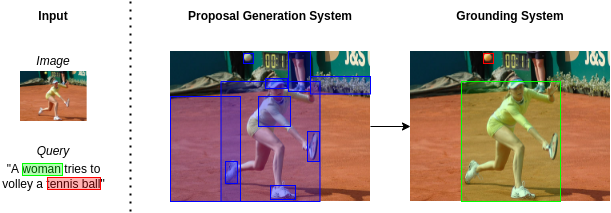
\includegraphics[width=.8\textwidth]{figures/two-stage-approach.png}
  \caption[Two stage approach]{
    The two stage approach. The grounding system receives a set of
    proposel extracted by a proposal generation system and, given the
    query, it aligns entities in query with (fixed) set of proposal.
  }
  \label{fig:two-stage-approach}
\end{figure}

Even if the approach seems very promising, it is not exempt from some
problems. As reported in \cite{yang2019fast} ``the propose-and-rank
two stage framework is flawed in at least two major ways''. First of
all, if none of the region candidates of the first stage hits the
ground truth region, the whole framework fails no matter how good the
second ranking stage could perform. Note that a hit is considered
successful if any of the proposals overlap the ground truth by more
than fifty percent in term of intersection over union (IoU). Secondly,
they argue that the process can be optimized by focusing on relevant
bounding boxes which are often a small number (2-5), instead of waste
lot of resources by computing thousands of proposal and then rank them
down to a list.

However, the highlighted problems highly depends on chosen proposal
extractor/object detector. Consider, for example, the problem of
hitting the ground truth with at least one bounding box. Given an
image $\bm{I}$ and $\bm{b}'$ a ground truth bounding box, if we
employee a very simple (yet extremely inefficient) proposal extractor
such us the one who generates $\calP^*_{\bm{I}}$ the set of all
possible bounding boxes in $\bm{I}$, then, by construction we have
that $b' \in \bm{B}$. Hence, the more proposals we consider, the
better we overlap with $\bm{b}'$. However, this solution is bound by
time and memory constraints, but fortunately we do not need to
generate all possible proposals. Indeed, only a small subset of all
solution are required to hit the ground truth bounding box. Thanks to
powerful object detection system we can recognize relevant objects in
image and focus only on those proposals.

Practically, we proved (Sec.~\ref{subsec:num-of-proposals}) that with
$100$ bounding boxes and Faster-R CNN with Bottom-Up Attention
\cite{sharma2020understanding} as object detector, we obtain a
coverage which is greater than 90\% on both two major dataset in the
field of study: Flickr30k and ReferIt.

The second problem instead is partially solvable because the system,
in order to perform its classification task, needs to consider all the
extracted proposal. However, the first stage can be precalculated and
cached for the second stage, drastically reducing the required
resources at training time. At inference time, instead, we need to run
both the object detector and the model without the possibility to
reduce computational time.

\newthought{The one stage approach}, outlined in
Fig.~\ref{fig:one-stage-approach} relies on a single stage for
computing the solution. The model should learn to both extract and
fuse visual and textual information in order to predict the best
bounding box in output, given in input an image and a sentence. 

The tight coupling provided by this approach may lead to higher
results with lower computational resources \cite{yang2019fast} and can
be used when there is no fixed set of categories \cite{sadhu2019zero},
but it raises some major issues. The main problem is the lack of data:
not all the visual grounding datasets are suitable for training an
object detector. Secondly, the model requires an high number of
parameters, and because of that the training requires significant
computing resources \cite{rigoni2021better}.

\begin{figure}
  \centering
  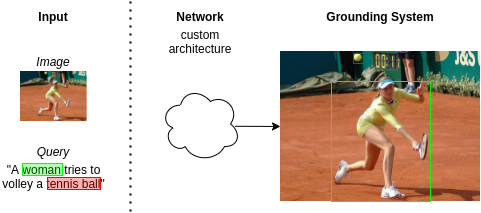
\includegraphics[width=.8\textwidth]{figures/one-stage-approach.png}
  \caption[One stage approach]{
    The one stage approach. The grounding system receives features
    encoded by a custom network with jointly process visual and
    textual features.
  }
  \label{fig:one-stage-approach}
\end{figure}

\section{Fully/Weakly/Self/Un-Supervised Settings}

Supervised classification and regression are two example of tasks that
in machine learning have archived great success. This happens because
machine learning models learn from ground truth annotation, however,
it is noteworthy that in many other tasks, like visual grounding, it
is difficult to get strong supervision due to the high cost of the
data-labeling process.

In visual grounding, large amount of annotations are required. Think
at the example in Fig.~\ref{fig:dog-playing-with-ball} along with the
sentence "A collie plays with a white ball in a field of green grass",
to perform phrase grounding task we need a lot of data: 
\begin{itemize}
  \item The image;
  \item The sentence;
  \item The annotations identifying queries in the sentence, for
  example ``the dog'', ``a ball'' and ``a field of green grass'';
  \item The annotations identifying entities in the image, i.e., the
  bounding box of the dog, of the ball and of the field with green
  grass.
  \item The annotations that links queries and boxes in the image,
  which are $\calO(mk)$ (fortunately, usually lower than that) where
  $m$ is the number of queries and $k$ the number of bounding box.
\end{itemize}
The collection of such amount of data needs a lot of effort and human
work to be carried out. Furthermore, because of the requirement of
human annotators, gathered data can be erroneous and biased. In
Sec.~\ref{sec:datasets} we extensively discuss two experiments (among
the others) that successfully collected such data and are became
State-of-the-Art datasets in phrase grounding.

It's straightforward to see that this approach cannot scale: larger
sets of annotations are exponentially difficult and expansive to
build. For this reason, researches usually redefine the phrase
grounding task under harder settings where less data are involved.
This is the case of weakly-supervised, or even, unsupervised visual
grounding. The Fig.~\ref{fig:full-weak-no-supervision} shows the
differences between the three supervised settings. In the first case,
a key information is available: the link between the query and the
correct box to ground. Under weakly supervised scenario instead, such
annotations are not available: we only know whether a query is linked
to an image, involving all its bounding box but not which is the
correct one. Under the unsupervised settings instead we do not have
access to ground truth, we have a corpus of text and a set of images
without link between them.

\begin{figure}[H]
  \centering
  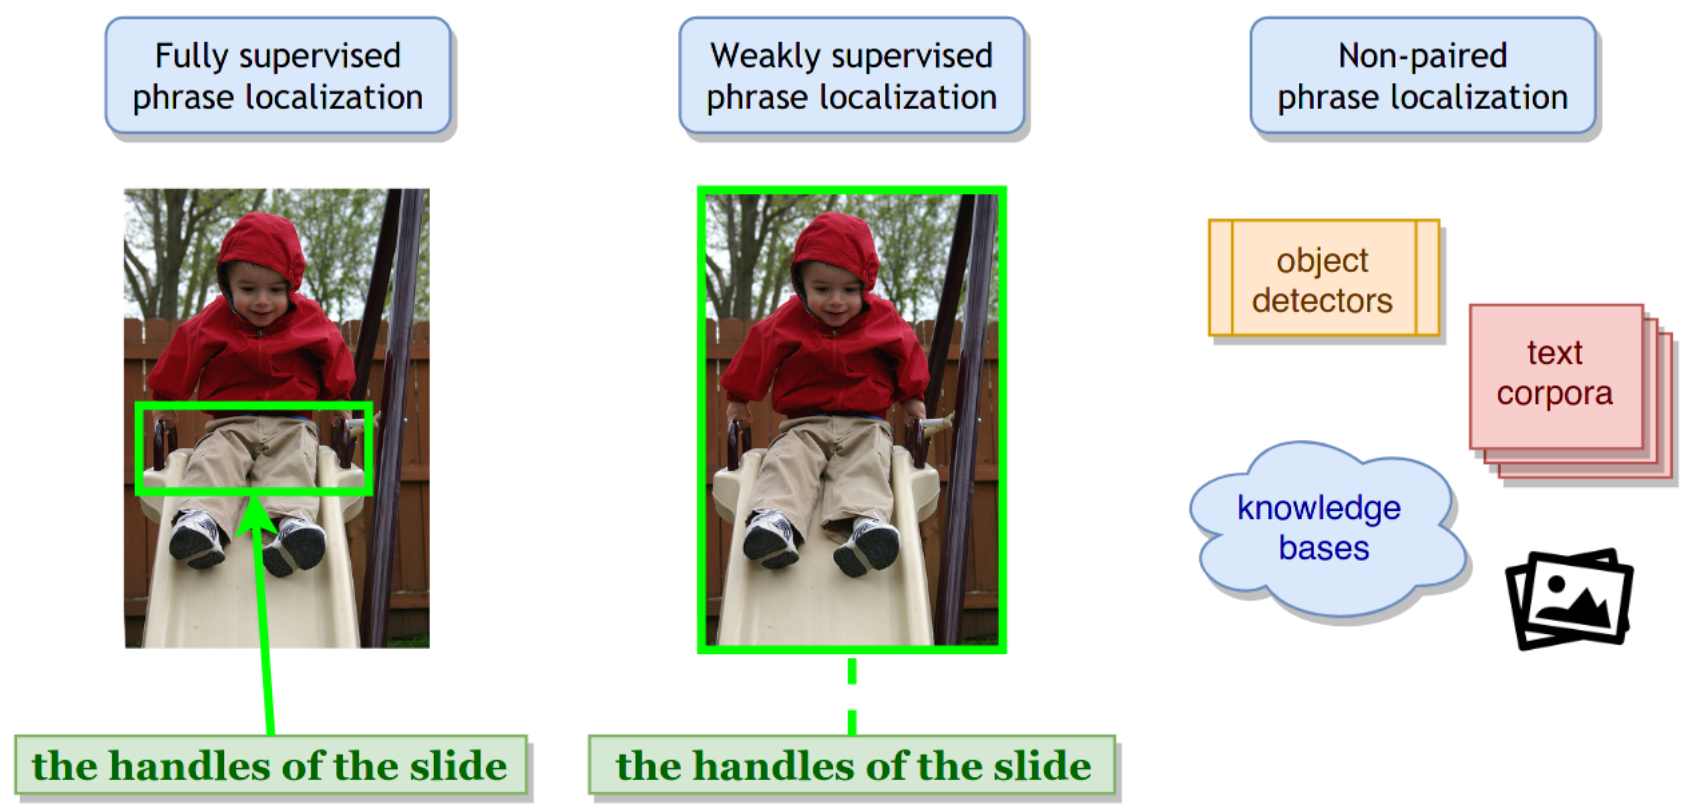
\includegraphics[width=.8\textwidth]{figures/full-weak-no-supervision.png}
  \caption[Differences between full, weak and no supervision]{
    Differences between full, weak and no supervision
    \cite{wang2019phrase}. Full supervision makes available the ground
    truth annotation on localization, while in weak supervision the
    ground truth involves only image-phrase pairs. Unsupervised
    settings instead do not provide ground truth.}
  \label{fig:full-weak-no-supervision}
\end{figure}

A simpler way to think at different supervision settings for phrase
grounding is by analogy with the ``match the shape'' game shown in
Fig.~\ref{fig:match-the-shape-game}, a game for children that make
them learn to recognize shapes like cube, cylinder, sphere and so on.
The game play is very simple: we are provided some pieces and we win
when all pieces fit in the hole on the board. Here, the model is
represented by the kid, and the input that in phrase grounding would
have been an image made by bounding box proposals and some queries are
the board along with holes and wooden pieces to fit on boards. Now,
consider a kid playing with two of such boards, the first has holes
for geometric shapes (cube, cylinder, sphere, etc.), while the second
has holes for tiny wooden animals (cow, cat, dog, fish, etc.). The
goal is to learn learn to fit pieces on boards. He starts without
knowledge, so he just tries. Pieces that fit in the holes will not
fall, so the kid understand whether a try is correct or not. After some
time of playing he has learnt where to put the cube and where to put a
cow. This is how the kid (or a grounding model) learns in fully
supervised scenario. Consider instead the scenario where the kid plays
with this two board, but he cannot try to put pieces in holes, he can
just ask whether a piece belongs to the board of shapes or animals. In
this much more complex way of playing, we give to kid only a weak
information: we tell him that a piece will fit on a board rather than
on the other, but we do not tell him which is the correct hole. This
is the weak supervision. In unsupervised settings instead the kid
cannot try neither to fit pieces on boards, nor to ask anything. He is
just left to itself.

\begin{figure}[H]
  \centering
  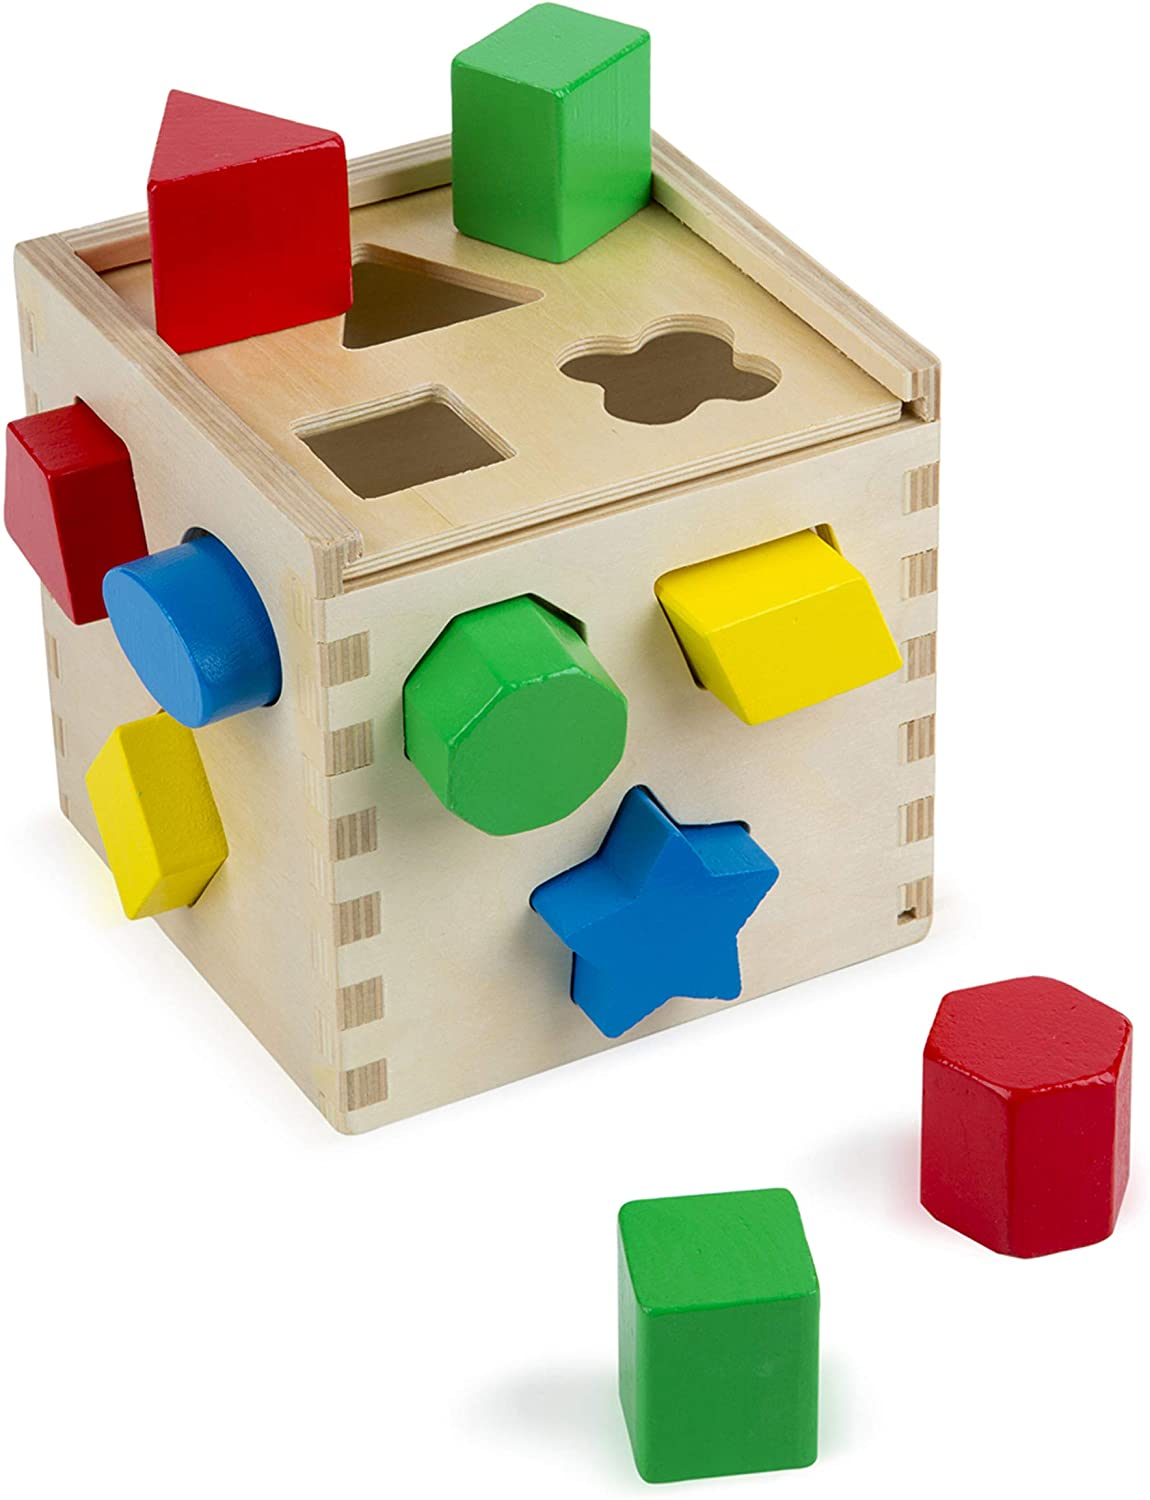
\includegraphics[width=.4\textwidth]{figures/match-shapes-game.jpg}
  \caption[Match the shape game]{
    Match the shape game. A kid game useful to learn to recognize
    shapes. The kid has to fit colored pieces in their respective
    holes.
  }
  \label{fig:match-the-shape-game}
\end{figure}

More abstractly, in fully supervised settings a training example
consists of two parts: a feature vector (or instance) describing the
event/object, and a label indicating the ground truth output.
Projected in phrase grounding this means knowing the map $\gamma :
\calI \times \calS \rightarrow 2^{\calQ \times \calB}$ that links the
ground truth bounding box $\bm{b}_i \in \calB$ with its query
$\bm{q}_j \in \calQ$.

Another form of supervision is the weak supervision. Broadly speaking,
weakly supervised learning is an umbrella term covering a variety of
architectures, all joint by the lack, degradation, or poorness of
data. Typically, three types of weak supervision are identified
\cite{zhou2018brief}.

\begin{itemize}
  \item The first is incomplete supervision (also known as semi
supervision \cite{rohrbach2016grounding}). Here, the ground truth is
available only for a (usually small) subset of training data, while
the other data remain unlabeled. Given an example $(\bm{I}, S, G)$, $G
= \{ (\bm{q}^{gt}_j, \bm{b}^{gt}_j) \}^{m'}_{j=1}$ where $m' \leq m$
with $m$ the number of noun phrases, in incomplete supervision we may
lack some ground truth in $G$.
  \item The second type is inexact supervision (also known as weak
supervision), i.e. only coarse-grained ground truth are given. In
phrase grounding inexact supervision means we have weak ground truth,
that is, we are given the pair $(\bm{I}, S)$ where we know only the
link between image and sentence but not the link between bounding
boxes and queries.
  \item The third type is inaccurate supervision, i.e. the given
labels are not always ground truth. In other words, some label
information may suffer from errors.
\end{itemize}

Inaccurate supervision is usually mixed with other settings because
the labelling procedure is carried out by human annotators which can
introduce errors.

\section{NLP and Part of Speech Tagging}

Part of Speech (POS) Tagging is a very basic and well known Natural
Language Processing (NLP) problem which consists of assigning to each
word of a text the proper morphosyntactic tag in its context of
appearance \cite{marquez2000machine}. It found applications in a wide
variety of of NLP tasks: as a preprocessing step to syntactic parsing,
in information extraction and retrieval (e.g. document classification
in internet searchers), text to speech systems, corpus linguistics,
etc. Due to intrinsic properties of languages, morphosyntactic tags
assigned to words highly depends on context in which words appear,
that is, in most cases words can be completely disambiguated  
by taking into account an adequate context. Furthermore, there are
even cases in which the ambiguity is non-resolvable using only
morphosyntactic features of the context, and require semantic and/or
pragmatic knowledge. For instance, in the sample sentence ``Yesterday
I read the paper'' the word \textit{read} is disambiguated as a past
simple because the word \textit{yesterday} at the beginning of the
sentence. Without context, the POS tagger can tag \textit{read} also
as a present or past participle.

Starting with the pioneer tagger \textsc{Taggit} developed by B. B.
Greene \etal{} in 1971, used for an initial tagging of the Brown
Corpus (BC), a lot of effort has been devoted to improving the quality
of the tagging process in terms of accuracy and efficiency. The
variety of existing taggers boils down to three main categories
according to the kind of knowledge they use. 

Systems that hardcode a set of rules (or constraints) written by
linguists belongs to the linguistic approach. The number of rules used
by such systems may vary from few hundreds to several thousand, and
their design usually requires years of labor. Moreover, they are hard
to scale to different set of data. For these reason, such systems did
not have a great diffusion and led to the development of other families that involves limited amount of human effort.

One of the most explored approach is the statistical family.
Basically, it disambiguates words by applying a statistical model
built on language. The model encodes information as a set of
co-occurrence frequencies for different kinds of linguistic phenomena.
For the acquisition of statistical data usually is used the n-gram
model, where the probability of sequence of length $n$ is estimated
from its occurrences in the training corpus. Usual models involved in
POS tagging instance $n$ to 2 or 3, i.e., possible sequences of two or
three consecutive tags (bi-grams or tri-grams). The tagging of new
example is done by estimating the tag sequence with high probability
based on the statistical model. This is roughly the technique followed
by the widespread Hidden Markov Model taggers. Based on similar idea,
the Baum-Welch re-estimation algorithm tries to reduce the amount of
training data needed to estimate the model. Recent works in this
field, instead of using a single n-gram model, combine different order
n-grams, morphological information, long-distance n-grams, or
triggering pairs.

According to \cite{marquez2000machine}, machine learning family
includes models which exploit more complex information than a n-gram
model. For example, Brill \etal{} learn in a machine learning fashion
a set of transformation rules with the goal to repair errors committed
by a most-frequent-tag tagger. Others acquire Constraint Grammar rules
from tagged corpora or apply instance-based learning. Promising
approaches explore decision trees induced from tagged corpora combined
with other statistical and linguistic information.

\subsection{POS tags}

POS tags were originally defined in \cite{marcus1993building} on the
Penn Treebank corpus as a comprehensive list of tags for words,
including noun, adjective, verb tenses and also symbols. The
Fig.~\ref{fig:pos-tags} shows the tags along with their description.

\begin{figure}
  \centering
  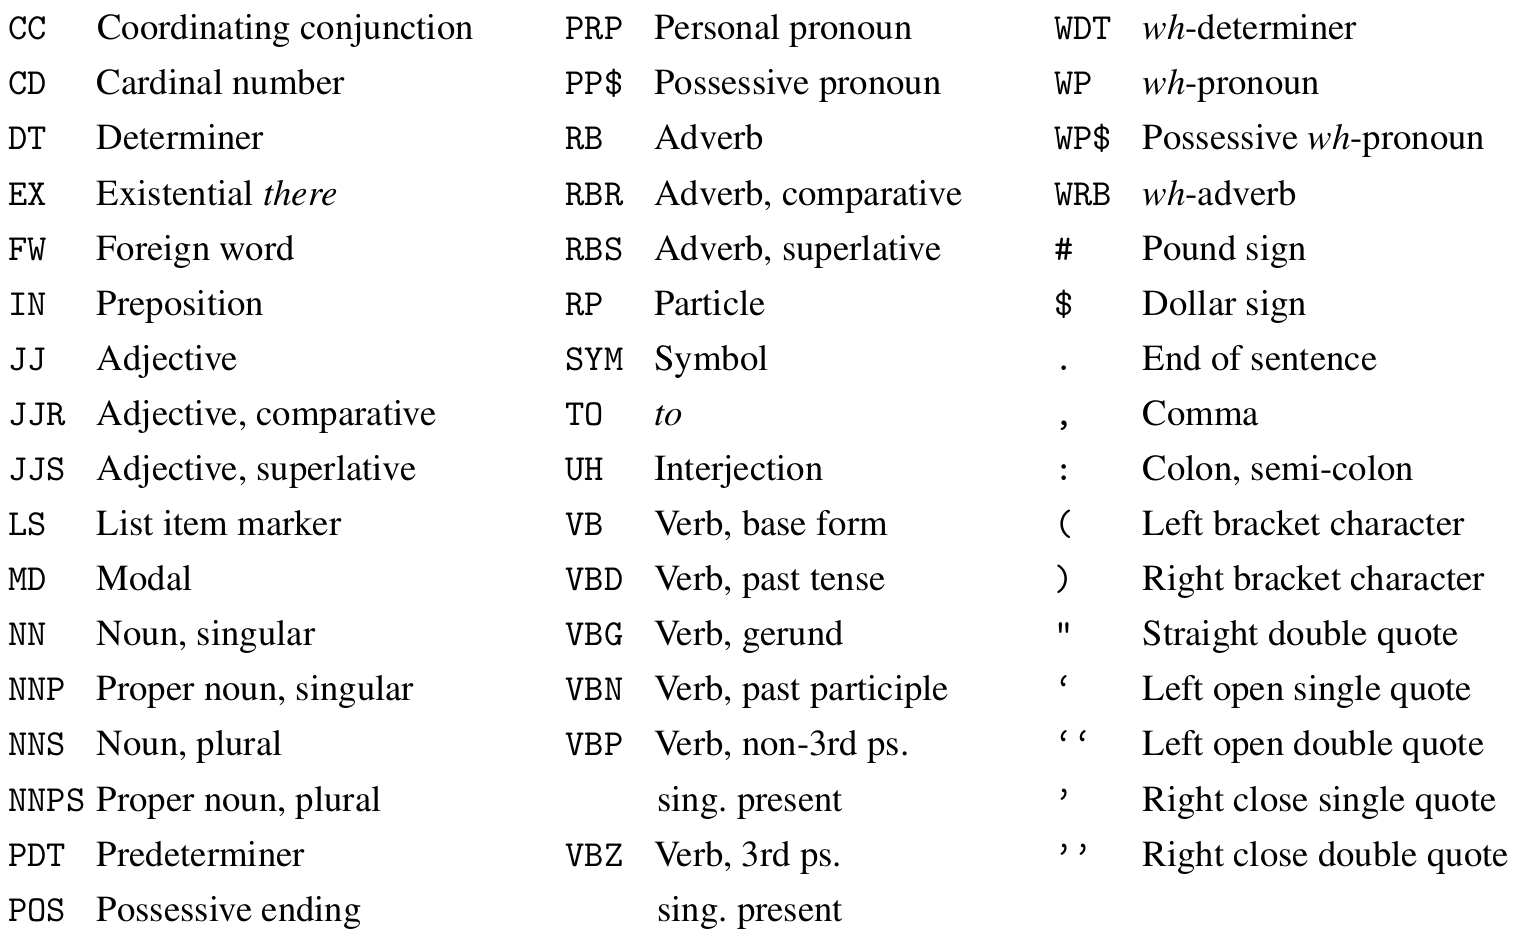
\includegraphics[width=.8\textwidth]{figures/pos-tags.png}
  \caption[POS tags]{POS tags of the Penn Treebank tag set \cite{marcus1993building}}
  \label{fig:pos-tags}
\end{figure}

During years, many different annotation for standard of POS tagging
and dependency structure were developed, such us Stanford Dependencies
\cite{de2006generating, de2008stanford, silveira2014gold}, Google
universal part-of-speech tags \cite{lin2012syntactic} and the Interset
interlingua \cite{zeman2008reusable} for morphosyntactic tagsets.
Universal Dependencies (UD) \cite{nivre2016universal,
nivre2017universal} is a recent effort to achieve cross-linguistic
consistency of annotation, while still permitting language-specific
extensions when necessary. The UD annotation scheme uses a
representation in the form of dependency trees as opposed to a phrase
structure trees and makes available over $100$ treebanks for more than
$70$ languages. New Universal POS tags are listed in
Fig.~\ref{fig:upos-tags}.

\begin{figure}
  \centering
  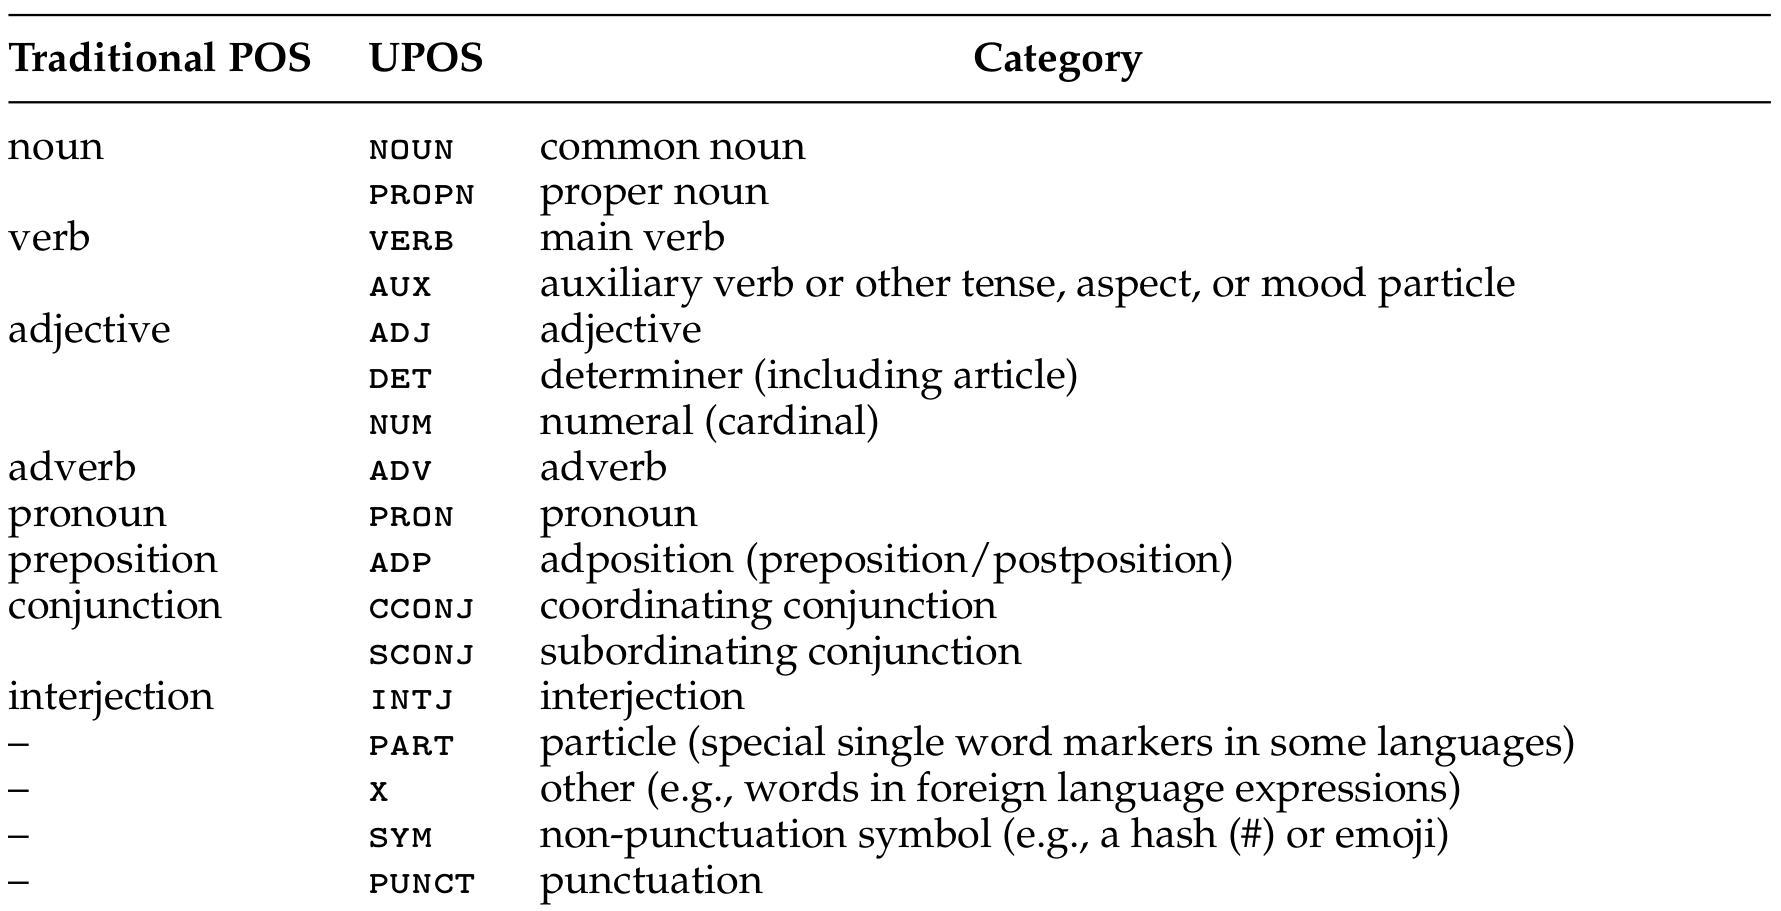
\includegraphics[width=0.9\textwidth]{figures/upos-tags.png}
  \caption[Universal POS tags]{Universal part-of-speech tags (UPOS) \cite{nivre2017universal}}
  \label{fig:upos-tags}
\end{figure}
 
\subsection{NLP Tools}

During years many good NLP tools were developed. The reasons are
twofold: first of all the availability of open-source dataset
simplified the training of such complex system, and secondly, NLP has
applications in many fields, from research to industry and even
government, thus, involving high demand for accurate and efficient
tools. Most famous and widely adopted appliances are CoreNLP
\cite{manning2014stanford}, \textsc{Flair} \cite{akbik2019flair},
spaCy\footnote{\href{https://spacy.io/}{https://spacy.io/}}, UDPipe
\cite{straka2018udpipe} and Stanza \cite{qi2020stanza}. Below we
discuss most relevant projects, highlighting their pro and cons. For a
detailed comparison between some NLP tools please refer to
\cite{schmitt2019replicable}.

\subsubsection{Standford CoreNLP}

Standford CoreNLP \cite{manning2014stanford} is the first NLP tool
developed for the mass adoption. CoreNLP was born at Standford
University in 2006 for internal usage and the released under an
open-source license in 2010. It implements a generic NLP pipeline from
tokenization through to coreference resolution. The motivations under
its development are:
\begin{itemize}
  \item To be able to quickly and painlessly get linguistic
  annotations for a text.
  \item To hide variations across components behind a common API.
  \item To have a minimal conceptual footprint, so the system is easy
  to learn.
  \item To provide a lightweight framework, using plain Java objects
  (rather than something of heavier weight, such as XML or UIMA's
  Common Analysis System (CAS) objects).
\end{itemize}
It tries to overcome problems of existing systems such us UIMA
\cite{ferrucci2004uima} and GATE \cite{cunningham2002gate} by allowing
the user to get ready in few minutes only knowing a little Java. For
example, Standford CoreNLP makes available an intuitive command line
interface and an easy way to write text annotators. Moreover, it
provides a simple concrete API which enables its usage from external,
existing systems. However, it does not attempt to provide multiple
machine scale-out (though it does provide multi-threaded processing on
a single machine).

Out of the box, Standford CoreNLP comes with many annotators and
supports all language encodings and various human languages like
English, Chinese, German, French and Arabic.

\subsubsection{SpaCy}

SpaCy defines itself an ``Industrial-Strength Natural Language
Processing Toolkit''. It is a free, open-source library for advanced
Natural Language Processing (NLP) in Python. It is designed
specifically for production use and helps you build applications that
process and ``understand'' large volumes of text. It can be used to
build information extraction or natural language understanding
systems, or to pre-process text for deep learning.

SpaCy implements many core features like tokenization, POS tagging,
dependency parsing, lemmatization, Sentence Boundary Detection (SBD),
Named Entity Recognition (NER), Entity Linking (EL), similarity, text
classification and rule-based matching. Practically, it is a swiss-army
knife for NLP pipelines.

\subsubsection{Stanza}

Stanza \cite{qi2020stanza} is a Python natural language
processing toolkit supporting many human languages. Its core features are:
\begin{itemize}
  \item From raw text to annotations. It features a fully neural
  pipeline which takes raw text as input, and produces annotations
  including tokenization, multi-word token expansion, lemmatization,
  part-of-speech and morphological feature tagging, dependency
  parsing, and named entity recognition.
  \item Multilinguality. Its architectural design is language-agnostic
  and data-driven, which allows us to release models supporting 66
  languages, by training the pipeline on the Universal Dependencies
  (UD) treebanks and other multilingual corpora
  \item State-of-the-art performance. They evaluate Stanza on a total
  of 112 datasets, and find its neural pipeline adapts well to text of
  different genres, achieving state-of-the-art or competitive
  performance at each step of the pipeline-
\end{itemize}
Additionally, Stanza features a Python interface to the widely used
Java CoreNLP package, allowing access to additional tools such as
coreference resolution and relation extraction. It is fully open
source and mdeks available pretrained models for all supported
languages and datasets available for public download.

\section{Recurrent Neural Network}
\label{sec:rnn}

A recurrent neural network (RNN) is a special type of an artificial
neural network (ANN) adapted to work for time series data or data that
involves sequences. Ordinary feed forward neural networks are only
meant for data points independent of each other while RNN introduces
the concept of ``memory'' that helps them store the states or
information of previous inputs to generate the next output of the
sequence by sharing weights.

An ANN with recursion can be easily modeled by the Eq.\ref{eq:rnn}:
\begin{equation}
  \label{eq:rnn}
  \bm{h}^{(t)} = f ( \bm{h}^{(t - 1)}, \bm{x}^{(t)} ; \bm{\theta} ),
\end{equation}
where $\bm{x}^{(1)}, \ldots, \bm{x}^{(\tau)}$ is the input sequence,
$f$ is the function that maps hidden units at time step $t - 1$ to
time step $t$ and $\bm{\theta}$ the parameters of $f$. The equation is
recurrent because the definition of $\bm{h}$ at time $t$ refers back
to the same definition at time $t - 1$. The process is visually
depicted in Fig.\ref{fig:rnn-with-unfold} \emph{(Left)}, where the
black square indicates a delay of a single time step. At this point
the problem is: how do we propagate our input through the RNN? Here
comes in the idea of unfolding. To unfold an RNN basically means to
unroll the cyclic circuit in a graph by explicitly applying the
function $f$ on $\bm{x}^{(t)}$, the input at time $t$, and
$\bm{h}^{(t-1)}$, the hidden state at time $t - 1$. RNN unfolding is
visually explained in Fig.\ref{fig:rnn-with-unfold} \emph{(Right)}.

\begin{figure}[H]
  \centering
  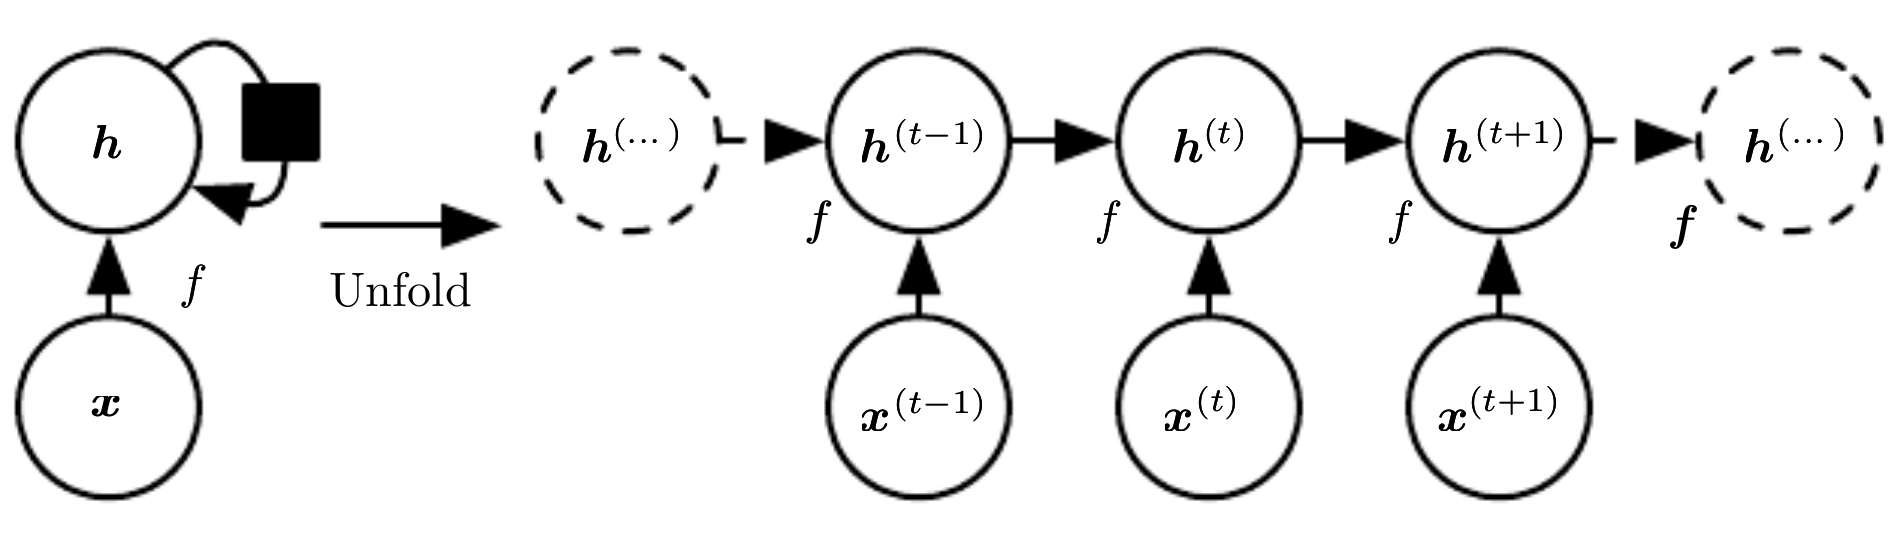
\includegraphics[width=.8\textwidth]{figures/rnn-with-unfold.png}
  \caption[Recurrent network circuit diagram and unfolded
    computational graph]{ A recurrent neural network with no outputs
    (typically RNNs add extra architectural features such as output
    layers that use information from the hidden state $\bm{h}$ to make
    predictions) \cite{goodfellow2016deep}. The left side of the
    picture shows an RNN that processes information from the input $x$
    by incorporating it into the state $\bm{h}$, that is passed
    forward through time. The black square indicates a delay of a
    single time step. In the right side the same RNN is shown, but
    here each node is now associated with one particular time
    instance. }
  \label{fig:rnn-with-unfold}
\end{figure}

When a RNN is trained to make predictions about the future with past
data, the network typically learns to use $\bm{h}^{(t)}$ as a lossy
summary, focusing on the relevant aspects of the past sequence of
inputs up to $t$. Such encoding of information, in general, is lossy
because an arbitrary sequence (with arbitrary length) $( \bm{x}^{(t)},
\bm{x}^{(t-1)}, \bm{x}^{(t-2)} , \ldots , \bm{x}^{(2)}, \bm{x}^{(1)}
)$ is mapped to a fixed length vector $\bm{h}^{(t)}$. The encoding may
selectively keep some insights of the past sequence with more
precision than other, depending on the training criterion. For
example, consider statistical language modelling, if the RNN is
required to predict next word from just read words, then not all
information in the input require to be memorized.

Recurrent neural networks can be built in many different ways with
varying architecture. In literature emerged some successful RNNs
architecture with a well defined and non-casual structure, such us
Bidirectional RNN (Bi-RNN), Long Short-Term Memory (LSTM) and Gated
Recurrent Unit (GRU). Each RNN architecture has some pro and cons and
can be applied successfully to specific tasks.

\subsection{Bidirectional RNN}

Bidirectional RNNs are a combination of two RNNs, where one reads the
sequence from start to end wrt time, while the other is reversed,
i.e., it moves backwards. Those networks have been applied
successfully when the output we want to predict depends on the whole
input sequence. A striking example of successful application for this
technique is speech recognition. Here, the correct interpretation of a
phoneme from sound may depend on the next few phonemes and potentially
may even depend on the next few words. The disambiguation of some
words may require past and future information. The same holds for
handwriting recognition and bioinformatics.

Such ability to work with past and future information implies that
Bi-RNNs cannot work with real-time sequences as future input are not
available.

\subsection{Gated RNN (LSTM and GRU)}
\label{subsec:gated-rnn}

Being able to work with long term dependencies is crucial for many
applications: think, for example, to a dialogue system which should
remember previous parts of the speech on order to keep on with the
dialogue.

Unfortunately, RNNs and long term dependencies yield a mathematical
challenge, namely gradient vanishing or gradient exploding. I.
Goodfellow \etal{} in \cite{goodfellow2016deep}, highlight this
problem:

\begin{quote}
  Even if we assume that the parameters are such that the recurrent
  network is stable (can store memories, with gradients not
  exploding), the difficulty with long-term dependencies arises from
  the exponentially smaller weights given to long-term interactions
  (involving the multiplication of many Jacobians) compared to
  short-term ones.
\end{quote}

One way to tackle this problem is to word at with multiple resolution
on time. Long-term dependencies mey be handled designing a model that
operates in some parts on fine-grained time scales and deals with
small details, while other parts works at coarse time scales. In this
settings, information from the distant past can flow more efficiently
to the present.

In literature, many ways are available for working both fine and
coarse time scales. These include the addition of 
\begin{enumerate*}[label=(\roman*)]
  \item special connections with the ability to skip steps in time, 
  \item new units, namely ``leaky units'', that integrate signals with
  different time constants, and 
  \item the removal of some of the connections used to model
  fine-grained time scales.
\end{enumerate*}

Like leaky units, gated RNNs are based on the idea of creating paths
through time that have derivatives that neither vanish nor explode.
For leaky units connection weights remain fixed for each time step,
while Gated RNNs generalize this to connection weights and allow them
to change over time.

The architecture of leaky units enables the accumulation of
information (such as evidence for a particular feature or category)
over a long duration. However, once that information has been used, it
might be useful for the neural network to forget the old state. When
to forget the old state can be automatically learned by the network.

LSTM basically integrates the idea of self-loops to produce paths
where the gradient can flow for long durations with, the addition to
control weight on this self-loop conditioned on the context, rather
than fixed. Moreover, the self-loop gate is controlled by another
hidden unit, thus, adding the ability to the network to change the
time scale dynamically. Fig.~\ref{fig:lstm} illustrate the LSTM block
diagram. In an LSTM cell, the self-loop controls the flow of
information from input to output through three key components: a
forget gate, an external input gate and an output gate.

\begin{figure}
  \centering
  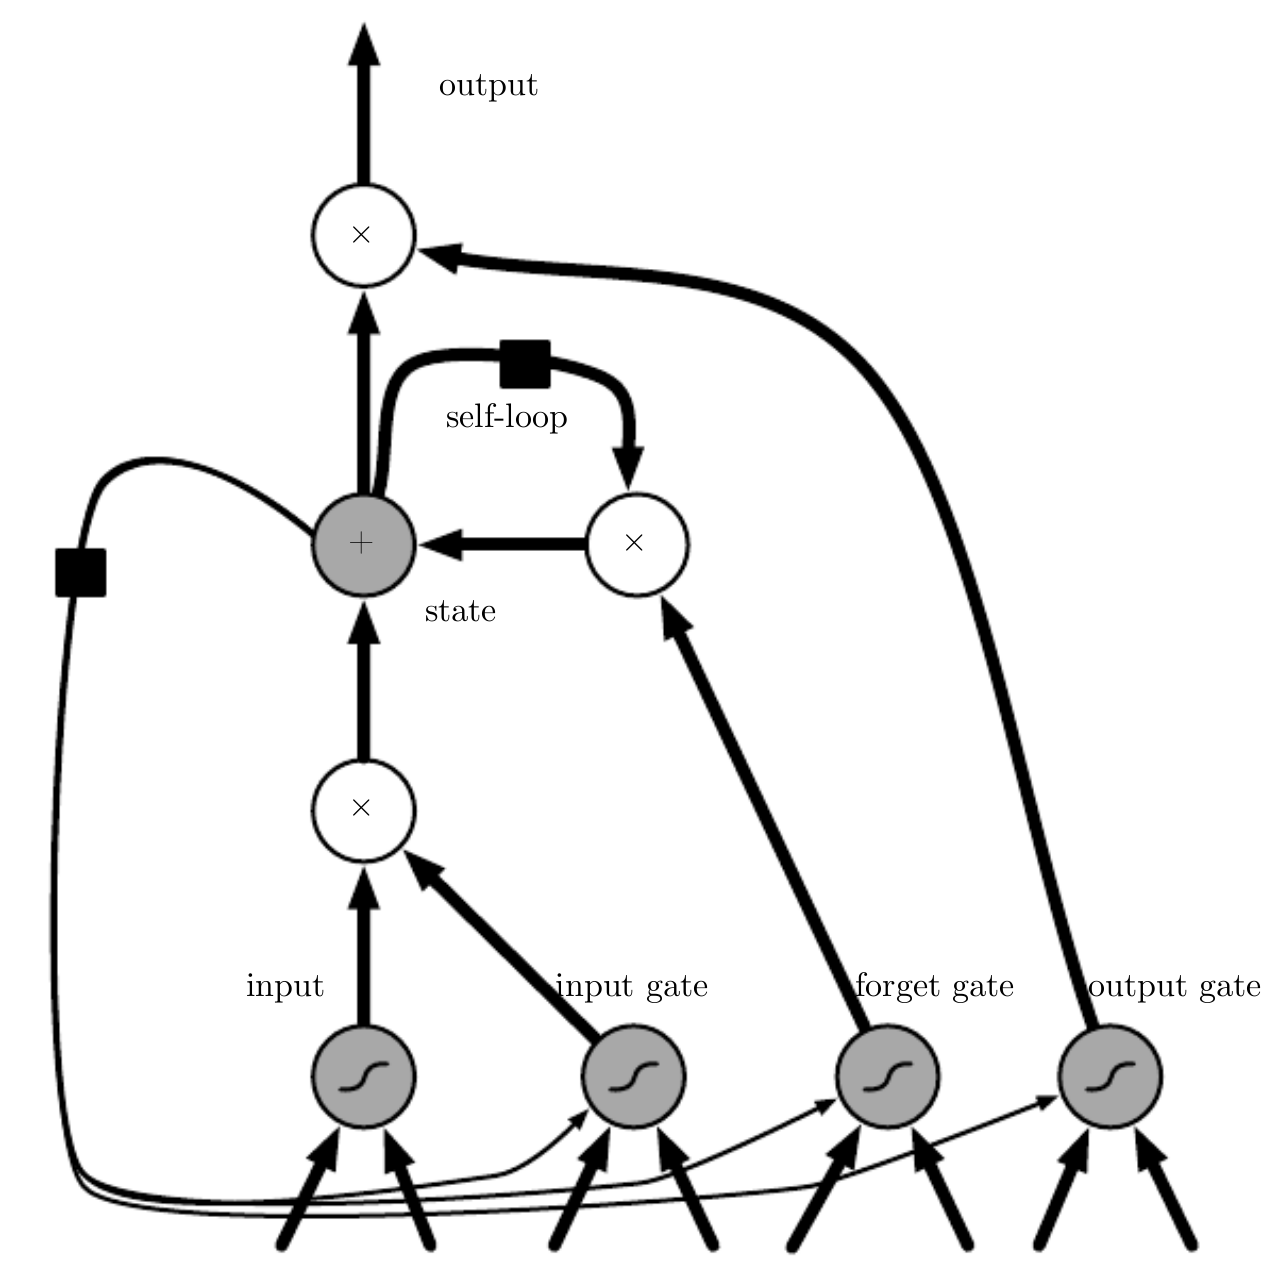
\includegraphics[width=.6\textwidth]{figures/lstm.png}
  \caption[Block diagram of the LSTM recurrent network cell]{ Block
    diagram of the LSTM recurrent network ``cell''
    \cite{goodfellow2016deep}. The state accumulates input stimuli
    which are conditioned by the input gate, while the forget gate
    controls whether to let slip the state. The output of the cell can
    be shut off by the output gate. The black square indicates a delay
    of a single time step. }
  \label{fig:lstm}
\end{figure}

Along with LSTM architecture, a simpler version was recently proposed
with the aim to simplify cells and speed-up computations: the gated
recurrent units (GRU). The behavior wrt LSTM is very similar, the only
difference is that a single gating unit simultaneously controls the
forgetting factor and the decision to update the state unit.

\section{Object Detection and Recognition Systems}
\label{sec:object-detection-recognition}

Object detection (OD) and object recognition (OR) systems are crucial
in a wide variety of everyday tasks such us face detection, image and
video databases information retrieval, surveillance applications,
driver assistance, self drive, robotics, automation and, specially in
vision tasks, it is a fundamental building block used to extract
information from images.

The primary essence of those systems can be broken down into two
parts: to locate objects in a scene such us by drawing a bounding box
around the object (object detection) and later to classify the objects
based on the classes it was trained on (object recognition). OD and OR
are Often used together and for this reason the name of two tasks is
usually used interchangeably. As for visual grounding
(Sec.~\ref{sec:two-stage-vs-one-stage}), we can group the
state-of-the-art detection systems in two main approaches: one stage
methods (YOLO -- You Only Look Once \cite{redmon2016you}, SSD --
Single Shot Detection \cite{liu2016ssd}) and two stage methods (R-CNN
\cite{girshick2014rich}, Fast R-CNN \cite{girshick2015fast}, Faster
R-CNN \cite{ren2015faster}). 

In the following sections, we briefly summarize those methods
discussing their main idea nd highlighting pro and cons.

\subsection{YOLO -- \emph{You Only Look Once}}
\label{subsec:yolo}

YOLO \cite{redmon2016you} is a state-of-the-art, real-time object
detection system which offers extreme levels of speed and accuracy.
YOLO treats object detection as a regression problem. It predicts
predicts both bounding boxes and class probabilities from full images
in a single pass, using a neural network. The process is optimized
directly on detection performance, in an end-to-end manner. Main
advantages over other architecture are the extreme speed and the
global image reasoning which allows to implicitly encode contextual
information about classes as well as their appearance. Hence, YOLO is
more likely to learn generalizable representations of objects because
of its global reasoning on image.

\subsection{SSD -- \emph{Single Shot Detection}}

SSD \cite{liu2016ssd} is another state-of-the-art method for detecting
objects in images using a single deep neural network. SSD divides the
image using a grid at multiple resolution and scale, then, for each
grid cell it detects objects in that region of the image. The
detection is performed by predicting the class and location of an
object within given cell by means of a convolutional and a
classification network. SSD obtains comparable results to other state
of the art detection system, while being able to run in little time as
its single pass on images. 

\subsection{R-CNN -- \emph{Regions with CNN}}

R-CNN \cite{girshick2014rich} is the first performant object detection
system ever built. It is composed by a two-stage architecture: in the
first step the Selective Search algorithm generates around 2000
category-independent region proposals for the input image, in the last
step instead it extracts a fixed-length feature vector from each
proposal using a CNN (hence the name R-CNN), and then classifies each
region with category-specific linear SVMs. The method shows
interesting results and can be applied also with scarce data
availability: the system can be pretrained and the fine-tuned. In
terms of computation time, R-CNN performs some expensive operations
required for greedy non-maximum suppression, among others, but on
relatively small inputs.

\subsection{Fast R-CNN}

The Fast R-CNN \cite{girshick2015fast} model was built to counter a
few drawbacks of the previous R-CNN model. In this approach, similar
to the previous, Selective Search is used to generate region proposals
but the input image is fed to a CNN and a convolutional feature map is
generated from it which is then used to identify the regions and
combine them into larger squares by using a RoI pooling layer. A
softmax layer is finally used to predict the class of the proposed
region.

\subsection{Faster R-CNN}
\label{subsec:faster-rcnn}

Unlike R-CNN and Fast R-CNN, Faster R-CNN \cite{ren2015faster} does
not use Selective Search which is a slow process. Instead, it allows
the network to learn the region proposals throught a separate network,
able to predict the region proposals. The predicted proposals are then
pooled into larger squares using the RoI pooling layer which is then
finally used to classify the image.

\section{Word Embeddings}
\label{sec:word-embeddings}

Being able to model and represent natural language features is a
relevant machine learning task that belongs to the natural language
processing field and has many applications, such us information
retrieval \cite{sanderson2010christopher}, document classification
\cite{sebastiani2002machine}, question answering
\cite{tellex2003quantitative}, named entity recognition
\cite{turian2010word}, and parsing \cite{socher2013parsing}.

Instead of treating words as atomic units where there is no notion of
similarity between words, as these are represented as indices in a
vocabulary, natural language information can be represented as
real-valued feature vectors through a semantic vector space, where
representation of words are learned for a predefined fixed sized
vocabulary from a corpus of text and the intrinsic quality of such a
set of word is evaluated by the distance or angle between pairs of
word vectors representations or by their various dimensions of
difference\cite{mikolov2013linguistic}. In light of this we can
formulate the definition for word embedding: 

\begin{quote}
  \textit{A word embedding is a learned representation for text where
  words that have the same meaning have similar representation.}
\end{quote}

With the years, literature explored different approaches for learning
good words representation: either using machine learning or
statistical approaches such us Latent Semantic Analysis. Both families
suffer significant drawbacks. LSA methods efficiently exploit
statistical information, but are unable to capture word analogies,
indicating a sub-optimal vector space structure. Methods like
skip-gram may do better on the analogy task, but suffer the lack of
statistical information since they train on separate local context
windows instead of on global co-occurrence counts.

\subsection{Word2Vec}

Word2Vec, introduced by T. Mikolov in \cite{mikolov2013efficient} and
then updated in \cite{mikolov2013distributed, mikolov2013linguistic},
is a statistical method for efficiently learning a standalone word
embedding from a text corpus. Word2Vec aims to learn significative
representations of words that capture semantic information. For this
reason, two different approaches are used: Continuous Bag-of-Words
(CBOW) and Continuous Skip-Gram Model. The CBOW model learns the
embedding by predicting the current word based on its context. The
continuous skip-gram model learns by predicting the surrounding words
given a current word. Both models, shown in
Fig.~\ref{fig:word2vec-learning-models} learn word representation
given their local usage scene. The context is defined by a window of
neighboring words and can be configured or fine-tuned. The quality of
these representations is measured in a word similarity task.

\begin{figure}
  \centering
  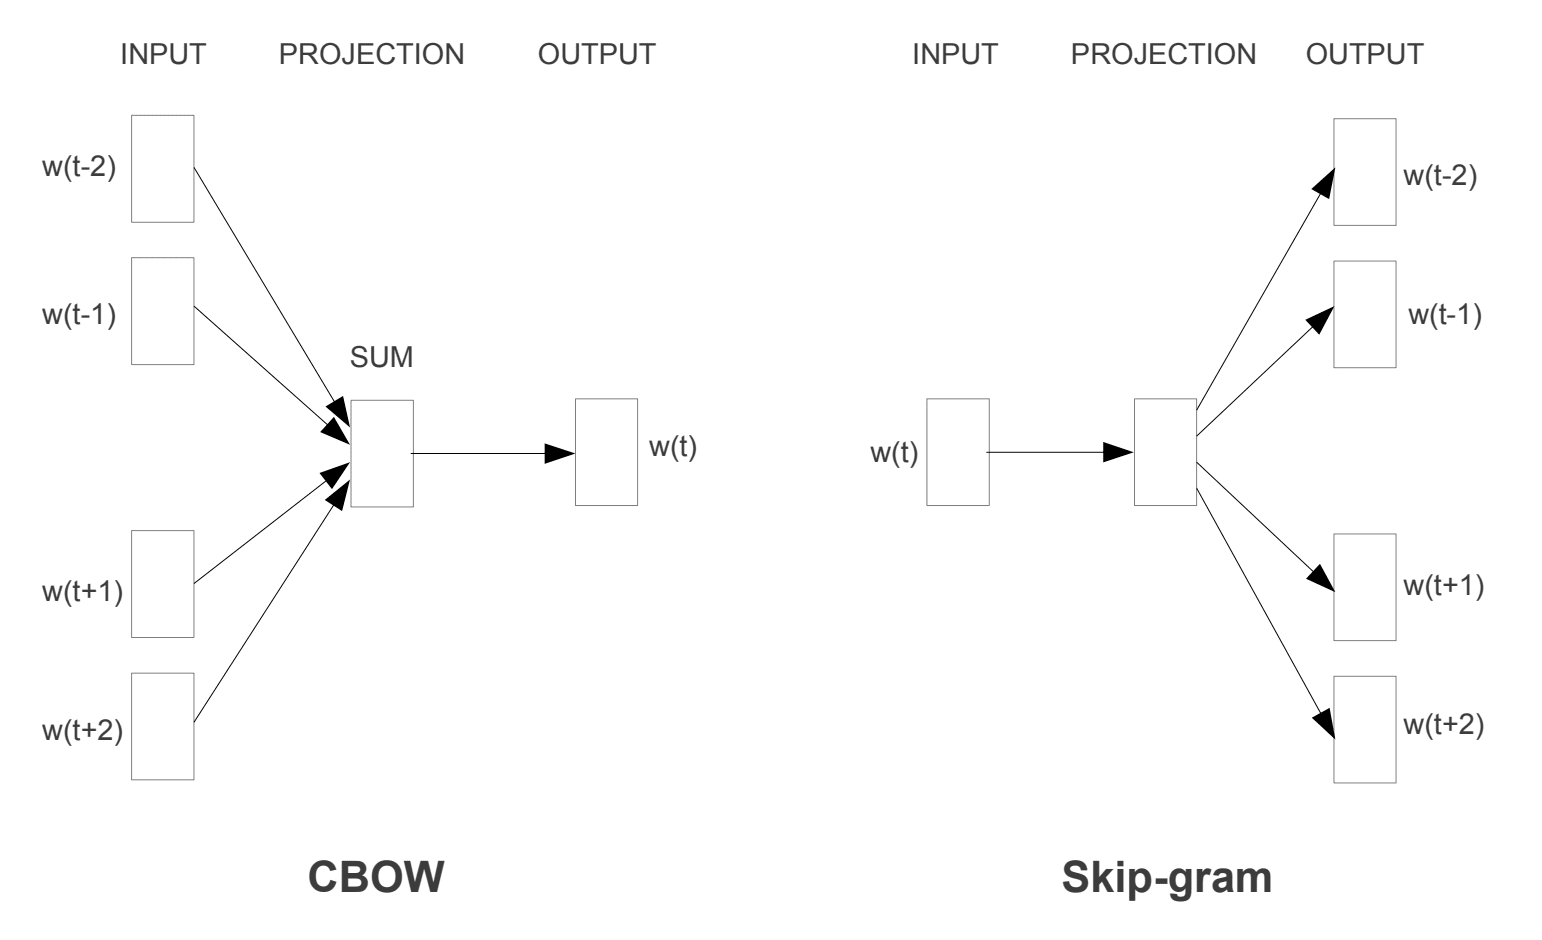
\includegraphics[width=0.8\textwidth]{figures/word2vec-training-models.png}
  \caption[Graphical representation of the CBOW model and Skip-gram model]{
    Graphical representation of the CBOW model and Skip-gram model
    \cite{mikolov2013exploiting}. In the CBOW model, the distributed
    representations of context (or surrounding words) are combined to
    predict the word in the middle. In the Skip-gram model, the
    distributed representation of the input word is used to predict
    the context.
  }
  \label{fig:word2vec-learning-models}
\end{figure}

The key benefit of the approach is that high-quality word embeddings
can be learned efficiently (low space and time complexity), allowing
larger embeddings to be learned (more dimensions) from much larger
corpora of text (billions of words). Also, Word2Vec perform
significantly better than LSA for preserving linear regularities among
words and LDA moreover becomes computationally very expensive on
large data sets.

\subsection{GloVe}

GloVe is an extension to the Word2Vec method for efficiently learning
word vectors, developed by J. Pennington \etal{} in
\cite{pennington2014glove}. The main goal of GloVe is to overcome
Word2Vec problems related to the lack of statistical information.
Rather than using a window to define local context, GloVe constructs
an explicit word-context or word co-occurrence matrix using statistics
across the whole text corpus. The result is a learning model that may
result in generally better word embeddings.

\subsection{Other methods}

\newthought{BERT} -- Bidirectional Encoder Representations from
Transformers is a relatively recent language representation model,
introduced by J. Devlin \etal{} in \cite{devlin2018bert}, designed to
pretrain deep bidirectional word representations from unlabeled text.
BERT exploit a deep transformer architecture instead of a traditional
recurrent neural network.

As outlined in \cite{gupta2020differences}, BERT has many difference
wrt traditional word embeddings: for example, it differs from Word2Vec
or GloVe because it produces multiple vector representations for the
same word, based on the context in which the word is used. For
example, in the sentences ``We went to the river bank'' and ``I need
to go to bank to make a deposit'', the word \textit{bank} produces
different embeddings in BERT for each sentence by taking into account
the context, while in Word2Vec or Glove, such word is represented by a
single, unique vector. Another key difference is that BERT explicitly
leverages on information involving the position of the word in the
sentence, which enhances the context dependence. Also, the input given
to the BERT model for predicting word embeddings needs to be a
sentence rather than a single word. This is because the BERT model
needs to know the context or the surrounding words before generating a
word vector. BERT can be used also in single-word mode to get
pre-computed static word vector (similar to Word2Vec or GloVe), but
this breaks the advantage of generating context dependent embeddings.

\section{Similarity Measures}

\subsection{Intersection over Union (IoU)}
\label{subsec:iou}

Given a pair of bounding box coordinates $(\bm{b}_i , \bm{b}_j)$, the
Intersection over Union (IoU), also known as Jaccard index, i.e.,
coefficient of similarity for two sets of data
\cite{jaccard1901comparative}, is an evaluation metric used mainly in
object detection tasks, which aims to evaluate how much the two
bounding box refer to the same content in the image
\cite{rigoni2021better, padilla2020survey}. Specifically, it is
defined as:
\[
  \iou(\bbox_i, \bbox_j) = \frac{| \bbox_i \inters \bbox_j |}{| \bbox_i \union \bbox_j |}
\]
where $| \bbox_i \inters \bbox_j |$ is the area of the box obtained by
the intersection of boxes $\bbox_i$ and $\bbox_j$ , while $| \bbox_i
\union \bbox_j |$ is the area of the box obtained by the union of
boxes $\bbox_i$ and $\bbox_j$. A conceptual explanation is given in
Fig.~\ref{fig:iou}. It is invariant to the bounding boxes sizes, and
it returns values that are strictly contained in the interval $[0, 1]
\in \Rset$, where $1$ means that the two bounding boxes refer to the
same image area, while a score of $0$ means that the two bounding
boxes do not overlap at all.

\begin{figure}
  \centering
  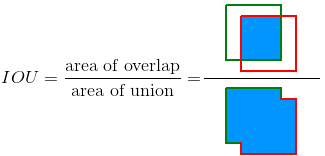
\includegraphics[width=0.6\textwidth]{figures/iou.png}
  \caption[Intersection over Union (IoU)]{Intersection over Union (IoU) \cite{padilla2020survey}}
  \label{fig:iou}
\end{figure}

\subsection{Pointing Game Metric}
\label{subsec:pointing-game-metric}

The pointing game can be considered an human evaluation metric
\cite{petsiuk2018rise} and was first introduced by J. Zhang \etal{} in
\cite{zhang2018top}. Given $(\bm{b}_i , \bm{b}_j)$ a pair of bounding
box, the pointing game metric defines a hit the highest saliency point
of $\bm{b}_i$ lies inside the $\bm{b}_j$, otherwise it is a miss.

The highest saliency point of a bounding box is usually defined
depending on the task and setting of the problem. For example, in the
phrase localization task, such point is the center of the bounding
box. In other cases, given an attention mask which localizes an object
in an image, the highest saliency point is the maximum point on the
attention mask.

\subsection{Cosine Similarity}

Cosine similarity is a metric used to measure how similar
representations are irrespective of their size (norm). Mathematically,
it measures the cosine of the angle between two vectors projected in a
multi-dimensional space:
\begin{equation}
  s_{\cos}(\bm{a}, \bm{b}) = \frac{\veca \cdot \vecb}{\normtwo\veca \normtwo\vecb},
\end{equation}
where $\veca \cdot \vecb$ is the dot product between two vectors and
$\normtwo\veca$ is the L2-norm of a vector.
